% Options for packages loaded elsewhere
\PassOptionsToPackage{unicode}{hyperref}
\PassOptionsToPackage{hyphens}{url}
%
\documentclass[
]{book}
\usepackage{amsmath,amssymb}
\usepackage{lmodern}
\usepackage{iftex}
\ifPDFTeX
  \usepackage[T1]{fontenc}
  \usepackage[utf8]{inputenc}
  \usepackage{textcomp} % provide euro and other symbols
\else % if luatex or xetex
  \usepackage{unicode-math}
  \defaultfontfeatures{Scale=MatchLowercase}
  \defaultfontfeatures[\rmfamily]{Ligatures=TeX,Scale=1}
\fi
% Use upquote if available, for straight quotes in verbatim environments
\IfFileExists{upquote.sty}{\usepackage{upquote}}{}
\IfFileExists{microtype.sty}{% use microtype if available
  \usepackage[]{microtype}
  \UseMicrotypeSet[protrusion]{basicmath} % disable protrusion for tt fonts
}{}
\makeatletter
\@ifundefined{KOMAClassName}{% if non-KOMA class
  \IfFileExists{parskip.sty}{%
    \usepackage{parskip}
  }{% else
    \setlength{\parindent}{0pt}
    \setlength{\parskip}{6pt plus 2pt minus 1pt}}
}{% if KOMA class
  \KOMAoptions{parskip=half}}
\makeatother
\usepackage{xcolor}
\IfFileExists{xurl.sty}{\usepackage{xurl}}{} % add URL line breaks if available
\IfFileExists{bookmark.sty}{\usepackage{bookmark}}{\usepackage{hyperref}}
\hypersetup{
  hidelinks,
  pdfcreator={LaTeX via pandoc}}
\urlstyle{same} % disable monospaced font for URLs
\usepackage{longtable,booktabs,array}
\usepackage{calc} % for calculating minipage widths
% Correct order of tables after \paragraph or \subparagraph
\usepackage{etoolbox}
\makeatletter
\patchcmd\longtable{\par}{\if@noskipsec\mbox{}\fi\par}{}{}
\makeatother
% Allow footnotes in longtable head/foot
\IfFileExists{footnotehyper.sty}{\usepackage{footnotehyper}}{\usepackage{footnote}}
\makesavenoteenv{longtable}
\usepackage{graphicx}
\makeatletter
\def\maxwidth{\ifdim\Gin@nat@width>\linewidth\linewidth\else\Gin@nat@width\fi}
\def\maxheight{\ifdim\Gin@nat@height>\textheight\textheight\else\Gin@nat@height\fi}
\makeatother
% Scale images if necessary, so that they will not overflow the page
% margins by default, and it is still possible to overwrite the defaults
% using explicit options in \includegraphics[width, height, ...]{}
\setkeys{Gin}{width=\maxwidth,height=\maxheight,keepaspectratio}
% Set default figure placement to htbp
\makeatletter
\def\fps@figure{htbp}
\makeatother
\setlength{\emergencystretch}{3em} % prevent overfull lines
\providecommand{\tightlist}{%
  \setlength{\itemsep}{0pt}\setlength{\parskip}{0pt}}
\setcounter{secnumdepth}{5}
\usepackage{booktabs}
\usepackage{titling}
\usepackage{pdfpages}
\pretitle{\begin{center}
\includepdf{images/logo-uel.png}}
\posttitle{\end{center}}
\usepackage{atbegshi}% http://ctan.org/pkg/atbegshi
\AtBeginDocument{\AtBeginShipoutNext{\AtBeginShipoutDiscard}}
\ifLuaTeX
  \usepackage{selnolig}  % disable illegal ligatures
\fi
\usepackage[]{natbib}
\bibliographystyle{plainnat}

\title{UNIVERSIDADE ESTADUAL DE LONDRINA\\
CCE - Centro de Ciências Exatas\\
DSTA - Departamento de Estatística\\
Apostila de Estatística\\
Prof.~M.e Eng. Felinto Junior Da Costa}
\author{}
\date{\vspace{-2.5em}Londrina, 14 de janeiro de 2023.}

\begin{document}
\maketitle

{
\setcounter{tocdepth}{1}
\tableofcontents
}
\hypertarget{section}{%
\chapter*{}\label{section}}
\addcontentsline{toc}{chapter}{}

\hypertarget{um-pouco-da-histuxf3ria}{%
\chapter{Um pouco da história}\label{um-pouco-da-histuxf3ria}}

\hypertarget{primeiros-levantamentos-estudos-e-publicauxe7uxf5es-demografia-e-aritmuxe9tica-poluxedtica}{%
\section{Primeiros levantamentos, estudos e publicações \& Demografia e aritmética política}\label{primeiros-levantamentos-estudos-e-publicauxe7uxf5es-demografia-e-aritmuxe9tica-poluxedtica}}

1086

O \emph{Domesday Book} \href{http://www.nationalarchives.gov.uk/education/resources/domesday-book/}{(link)}
foi encomendado em dezembro de 1085 por Guilherme, o Conquistador (\emph{King William I}), que invadiu a Inglaterra em 1066.

O primeiro esboço foi concluído em agosto de 1086 e continha registros de 13.418 assentamentos nos condados ingleses ao sul dos rios Ribble e Tees (a fronteira com a Escócia) com informações sobre terras, proprietários, uso da terra, empregados e animais cujo propósito básico era fundamentar a taxação.

\begin{figure}

{\centering 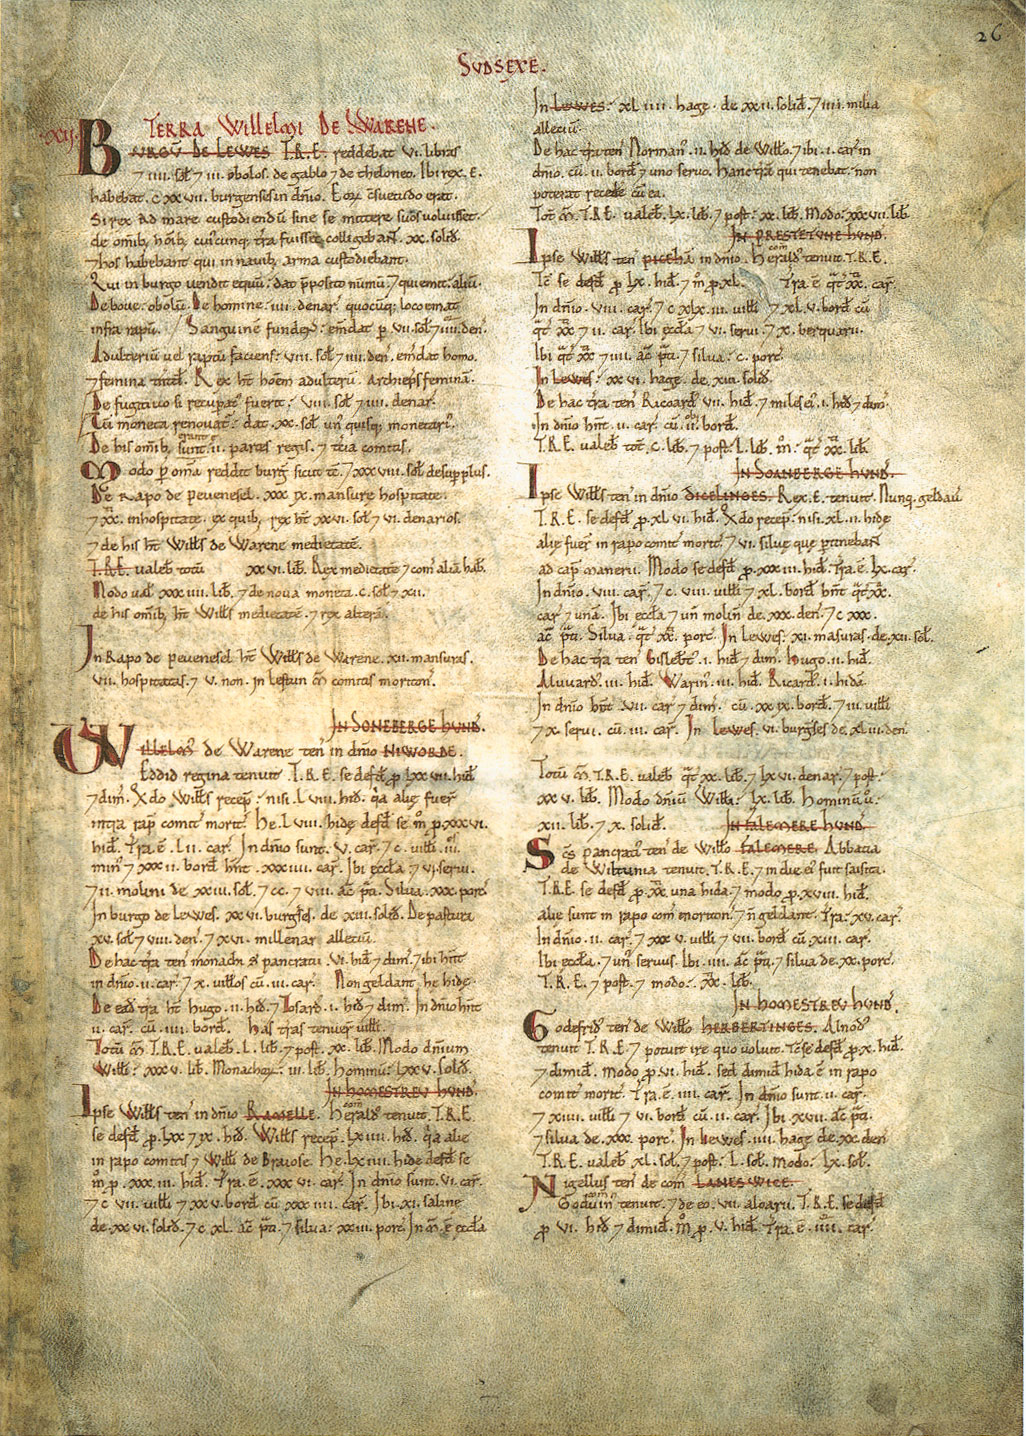
\includegraphics[width=0.75\linewidth]{images/domesday} 

}

\caption{Domesday Book}\label{fig:unnamed-chunk-3}
\end{figure}

1602

O dramaturgo inglês William Shakespeare usou a palavra \textbf{statists} (estadistas e, portanto, num sentido não relacionado com números ou matemática) no diálogo da Cena II de Hamlet \href{http://shakespeare.mit.edu/hamlet/full.html}{(link)}.

\begin{quote}
``Hamlet:
Cercado assim por tantas vilanias, mesmo antes de eu poder dizer o prólogo, representava o cérebro.
Sentei-me e escrevi com capricho nova carta. Já pensei, como os nossos estadistas, que é feio escrever bem, tendo insistido, até, em desaprendê-lo; mas, nessa hora muito bom me foi isso. Quererias saber
qual o conteúdo da mensagem?{[}\ldots{]}''
\end{quote}

1603

O negociante inglês John Graunt (1620-1674) substituiu a crença pela evidência em \emph{Natural and Political Observations Mentioned in a Following Index and Made upon the Bills of Mortality} (Observações naturais e políticas feitas sobre as notas de mortalidade).

Nesse trabalho, realizado com dados coletados das paróquias de Londres entre 1604 e 1660, Graunt tirou as seguintes conclusões: que havia maior nascimento de crianças do sexo masculino, mas havia distribuição aproximadamente igual de ambos os sexos na população geral; alta mortalidade nos primeiros anos de vida; maior mortalidade nas zonas urbanas em relação às zonas rurais.

\begin{figure}

{\centering 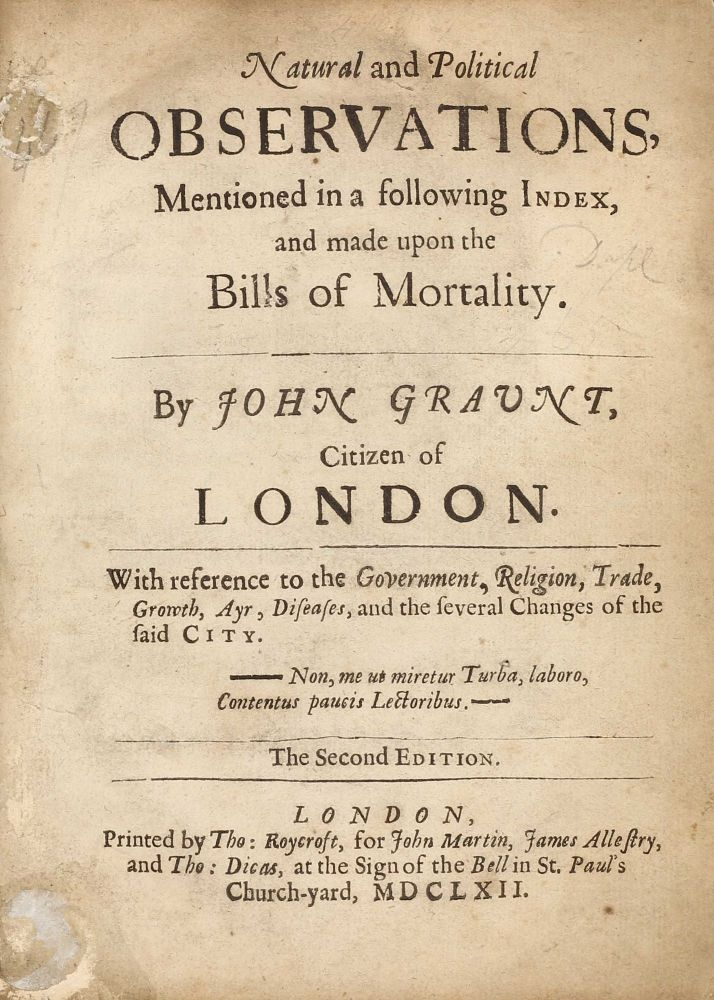
\includegraphics[width=0.75\linewidth]{images/graunt} 

}

\caption{Natural and Political Observations Mentioned in a Following Index and Made upon the Bills of Mortality (ed. de 1662)}\label{fig:unnamed-chunk-4}
\end{figure}

1660

Herman Conring (1606-1681), professor de filosofia, medicina e política da Universidade de Helmstadt (atual Alemanha), criou um curso de Ciência política em 1660, que descrevia e examinava as questões fundamentais do Estado. Nele a \textbf{estatística} passou a ser considerada como uma disciplina autônoma que tinha por objetivo a descrição das coisas do Estado.

1687

Em 1687 o economista e filósofo inglês William Petty (1623-1687) publicou \emph{Five Essays on Political Arithmetic} (Cinco ensaios sobre aritmética política), sugerindo ao governo inglês a criação de um departamento para registro de \textbf{estatísticas} vitais.

\begin{figure}

{\centering 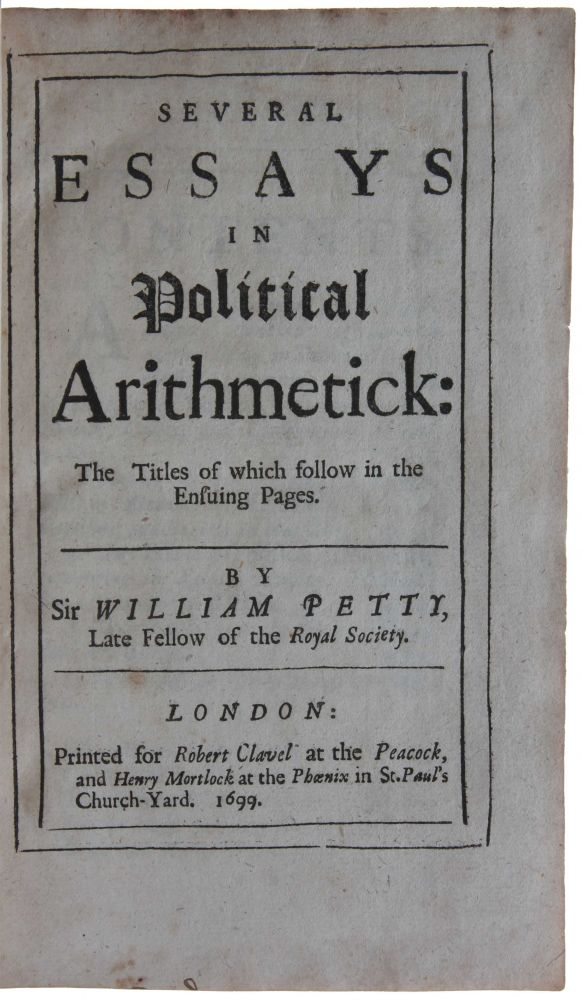
\includegraphics[width=0.75\linewidth]{images/petty} 

}

\caption{Several Essays in Political Arithmetick (ed. de 1699)}\label{fig:unnamed-chunk-5}
\end{figure}

O Capitão John Graunt e William Petty instituiram na Inglaterra um novo ramo de estudos denominado de \textit{Political arithmetic} (Aritmética política)

1693

O matemático e astrônomo inglês Edmond Halley (1656-1742) construiu em 1693, baseado em dados coletados na cidade (à época) alemã de Bresláu, uma \emph{Life Table} (Tábua de sobrevivência), um estudo que analisa as probabilidades de sobrevivência e morte em relação à idade.

\begin{figure}

{\centering 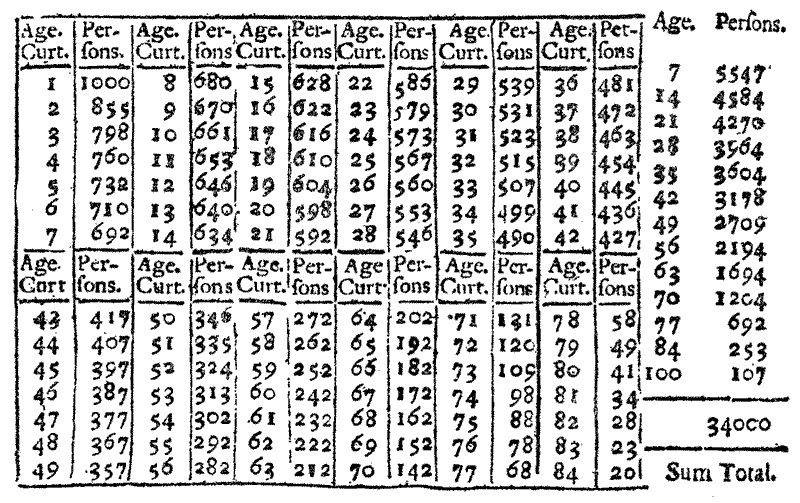
\includegraphics[width=0.75\linewidth]{images/halley} 

}

\caption{Halley’s life table (1693)}\label{fig:unnamed-chunk-6}
\end{figure}

1749

Com um sentido não relacionado com números ou matemática, a palavra \textbf{estatística} parece ter sido proposta pela primeira vez no século XVII, pelo historiador e professor alemão (à época Transilvânia) Martin Schmeitzel (1679-1747) da Universidade de Jena e, posteriormente adotada por seu aluno, (igualmente) historiador e jurista Gottfried Achenwall (1719-1772) em 1749, em \emph{Abriß der neuen Staatswissenschaft der vornehmen Europäischen Reiche und Republiken} (Esboço da nova ciência política dos nobres impérios europeus e repúblicas).

\begin{figure}

{\centering 
\includegraphics[width=0.75\linewidth]{images/gottfried} 

}

\caption{Abriß der neuen Staatswissenschaft der vornehmen Europäischen Reiche und Republiken (1749)}\label{fig:unnamed-chunk-7}
\end{figure}

1771

William Hooper usou a palavra \textbf{estatística} em sua tradução de \emph{The Elements of Universal Erudition}(Elementos da Erudição Universal) escrita por Jacob Friedrich Freiherr von Bielfeld (1717-1770).

Nesse livro, a \textbf{estatística} foi definida como a ciência que nos ensina o arranjo político de todos os estados modernos do mundo conhecido (mais uma veznum sentido não associado a números ou matemática).

\begin{figure}

{\centering 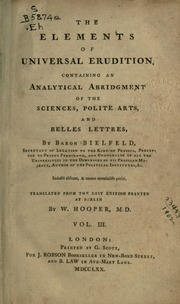
\includegraphics[width=0.75\linewidth]{images/hooper} 

}

\caption{The Elements of Universal Erudition  (1771)}\label{fig:unnamed-chunk-8}
\end{figure}

1790

O jurista e político escocês John Sinclair propôs que se realizasse uma detalhada pesquisa em 938 paróquias para elucidar a história natural e política de seu país (\emph{Statistics Accounts}). Essa pesquisa fazia parte de um projeto muito mais ousado: \emph{The Pyramid of Statistical Enquiry} (A Pirâmide da Pesquisa Estatística).

\begin{figure}

{\centering 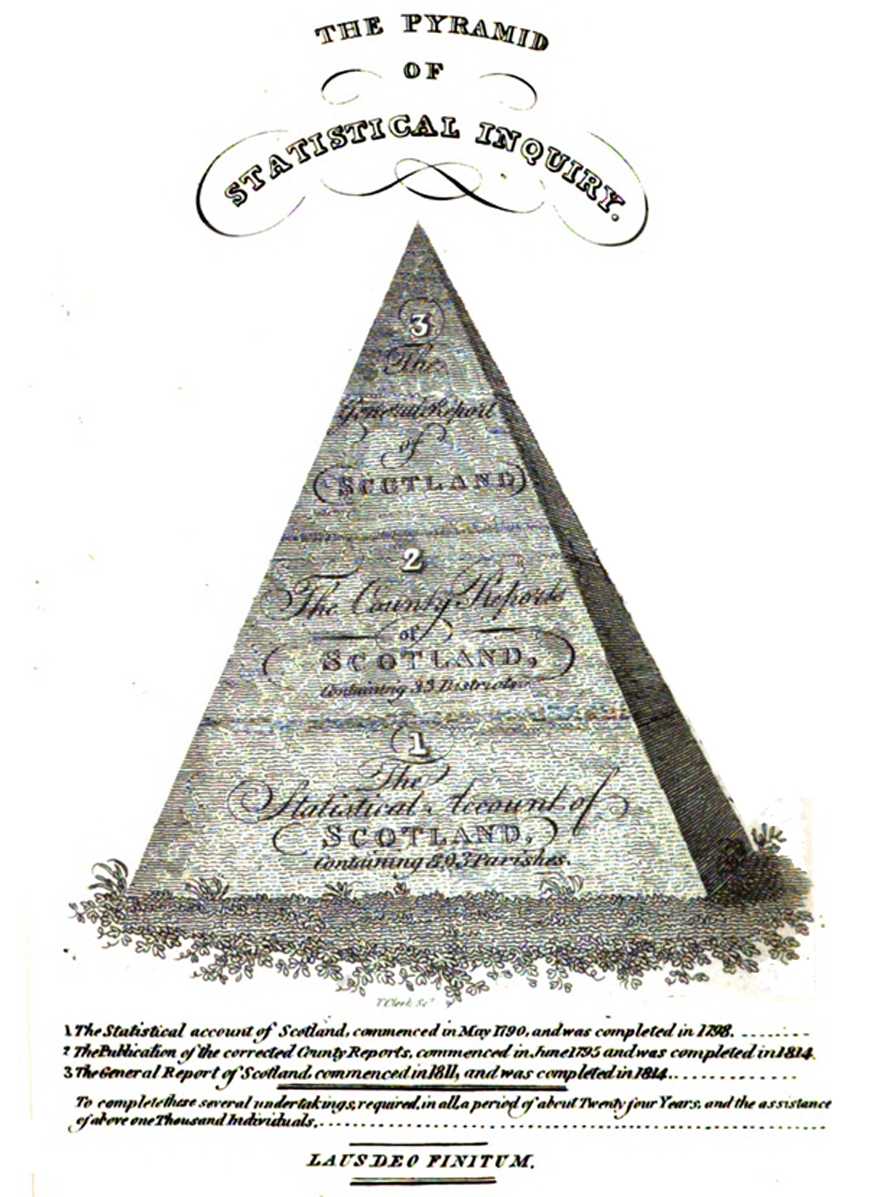
\includegraphics[width=0.75\linewidth]{images/sinclair} 

}

\caption{The Pyramid of Statistical Enquiry  (1814)}\label{fig:unnamed-chunk-9}
\end{figure}

1854

O médico inglês (considerado por alguns como o ``pai'' da epidemiologia moderna) John Snow (1813-1858) estudou a dispersão espacial dos casos de cólera em Londres e concluiu que sua causa residia na contaminação da água consumida (poço localizado na \emph{Broad Street}, no distrito do \emph{Soho}): \emph{Report to the Cholera Outbreak in the Parish of St.~James, Westminster during the Autumn of 1854} (Relatório sobre o surto de cólera na paróquia de St.~James, Westminster durante o outono de 1854).

\begin{figure}

{\centering 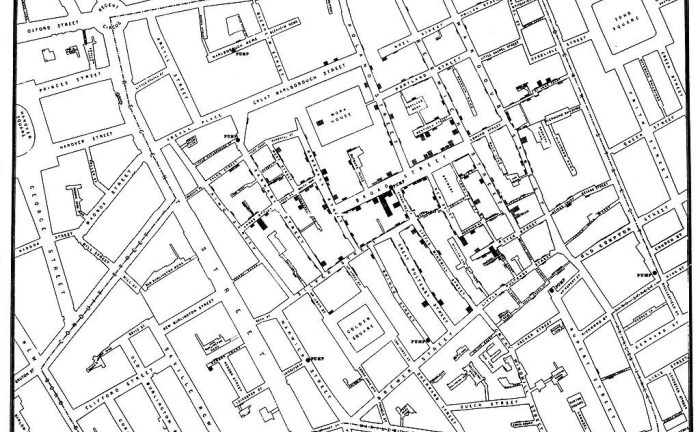
\includegraphics[width=0.75\linewidth]{images/london-1854-snow} 

}

\caption{Mapa dos casos de cólera (1854)}\label{fig:unnamed-chunk-10}
\end{figure}

\hypertarget{visualizauxe7uxe3o-de-dados-estudos-e-primeiras-publicauxe7uxf5es}{%
\section{Visualização de dados \& Estudos e primeiras publicações}\label{visualizauxe7uxe3o-de-dados-estudos-e-primeiras-publicauxe7uxf5es}}

1765

O teólogo e filósofo inglês Joseph Priestley (1733-1804) introduziu como inovação os primeiros gráficos com linha temporal, em que barras individuais eram usadas para visualizar o tempo de vida de uma pessoa e o todo pode ser usado para comparar a expectativa de vida de várias pessoas.

\begin{figure}

{\centering 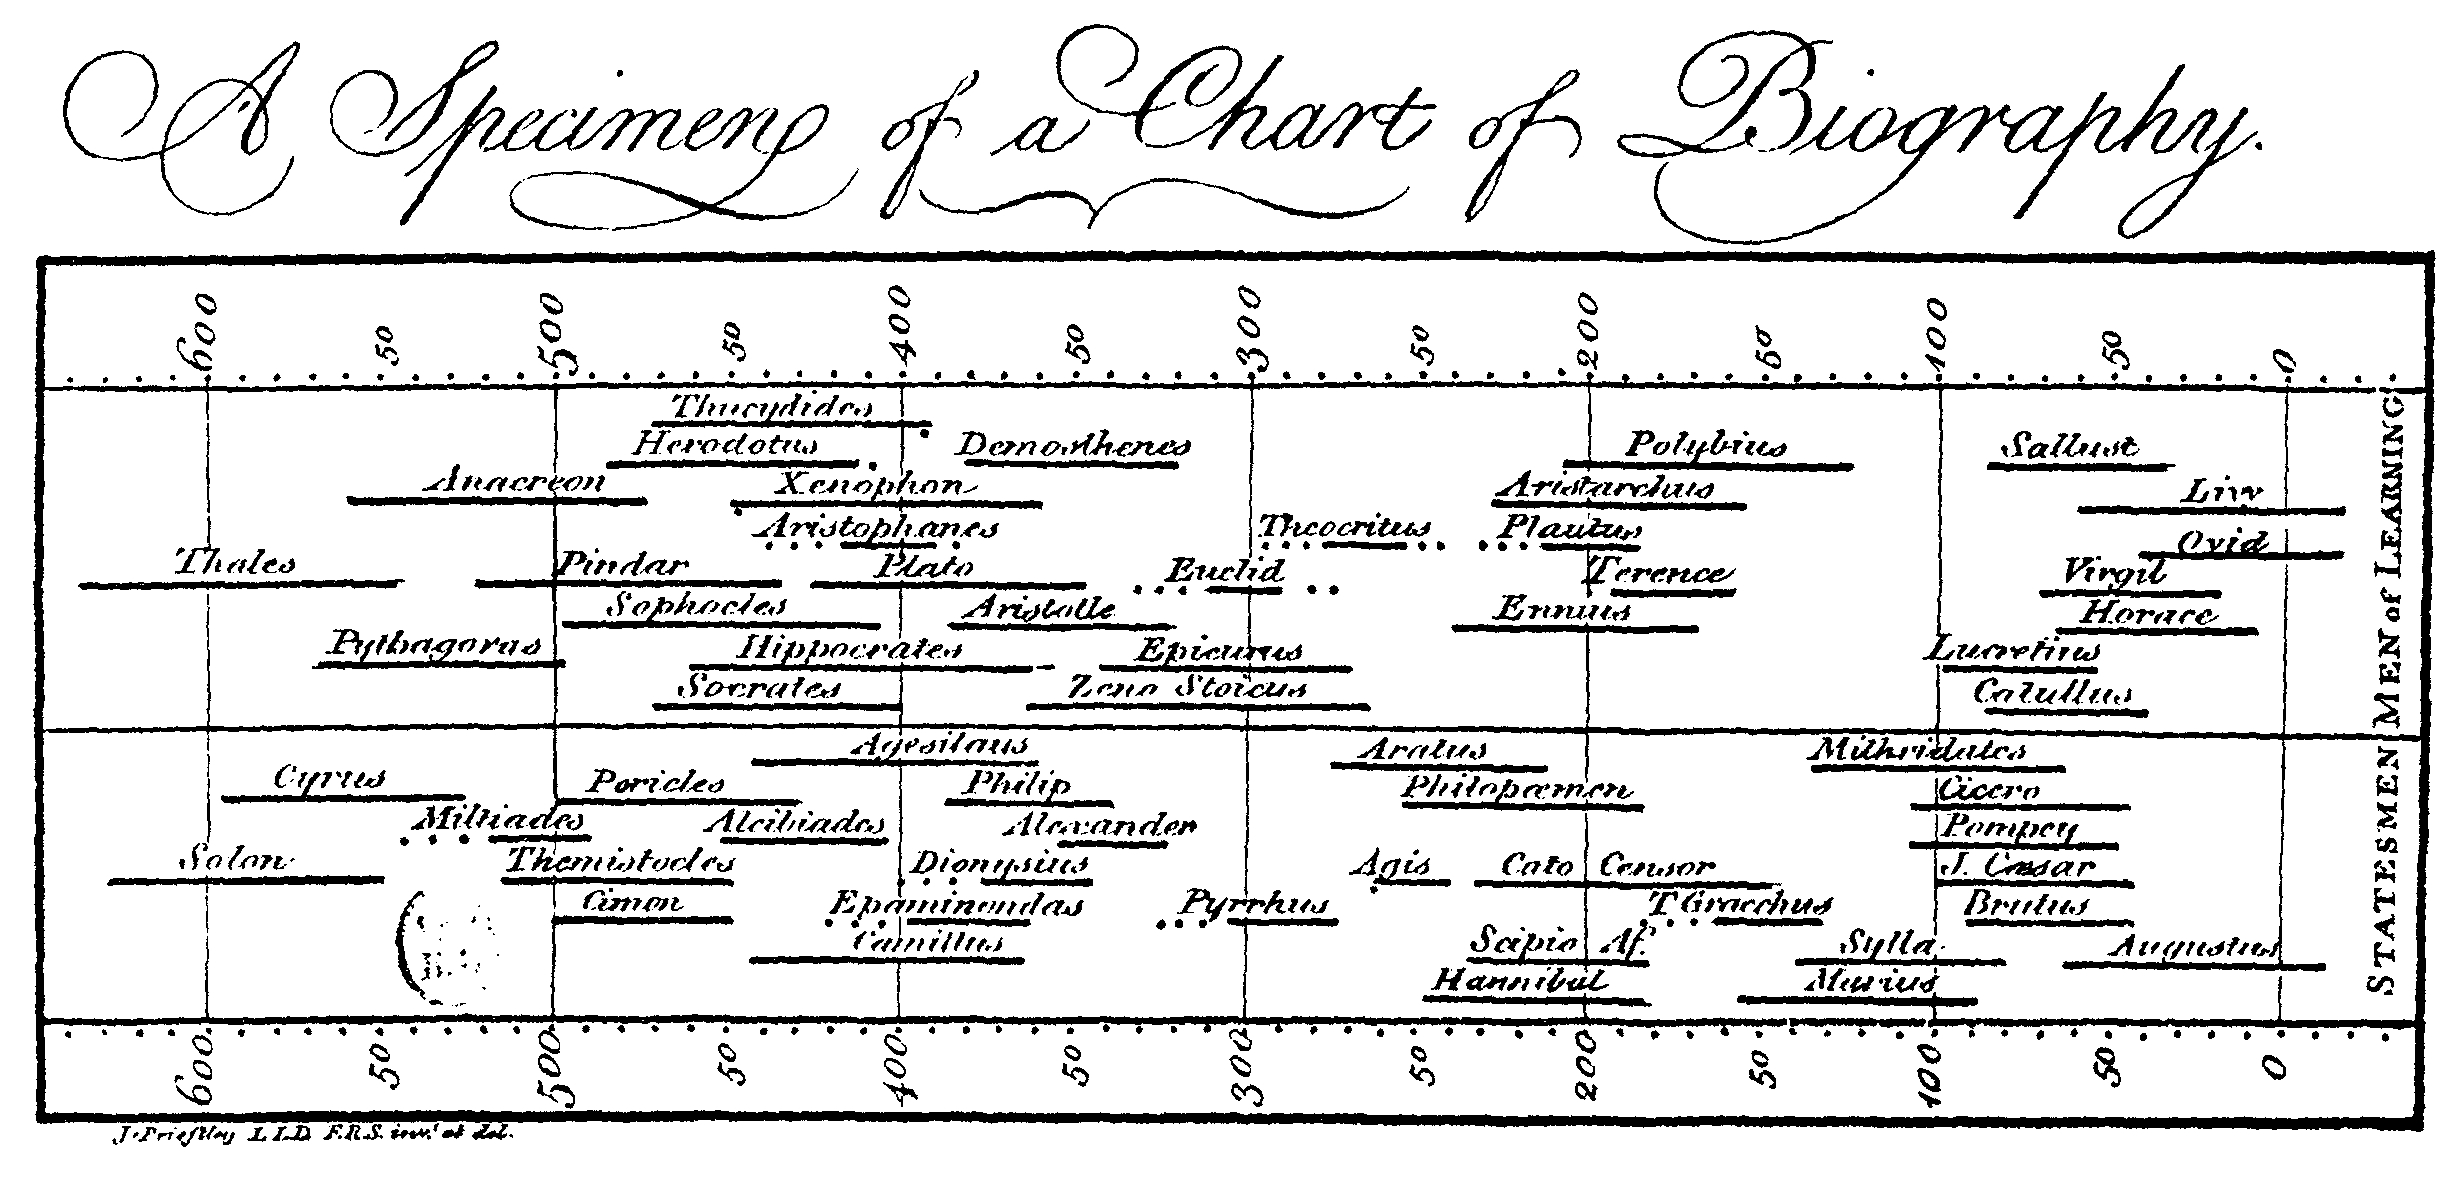
\includegraphics[width=0.75\linewidth]{images/priestley-timechart-1765} 

}

\caption{Expectativa de vida de diversas pessoas (1765)}\label{fig:unnamed-chunk-11}
\end{figure}

1786

O engenheiro e economista escocês William Playfair (1759-1823) é considerado comumente como fundador dos métodos gráficos para apresentação de estatísticas. Playfair concebeu vários tipos de diagramas para visualização de dados:

\begin{itemize}
\tightlist
\item
  em 1786, o gráfico de barras; e,
\item
  em 1801, o gráfico de setores.
\end{itemize}

\begin{figure}

{\centering 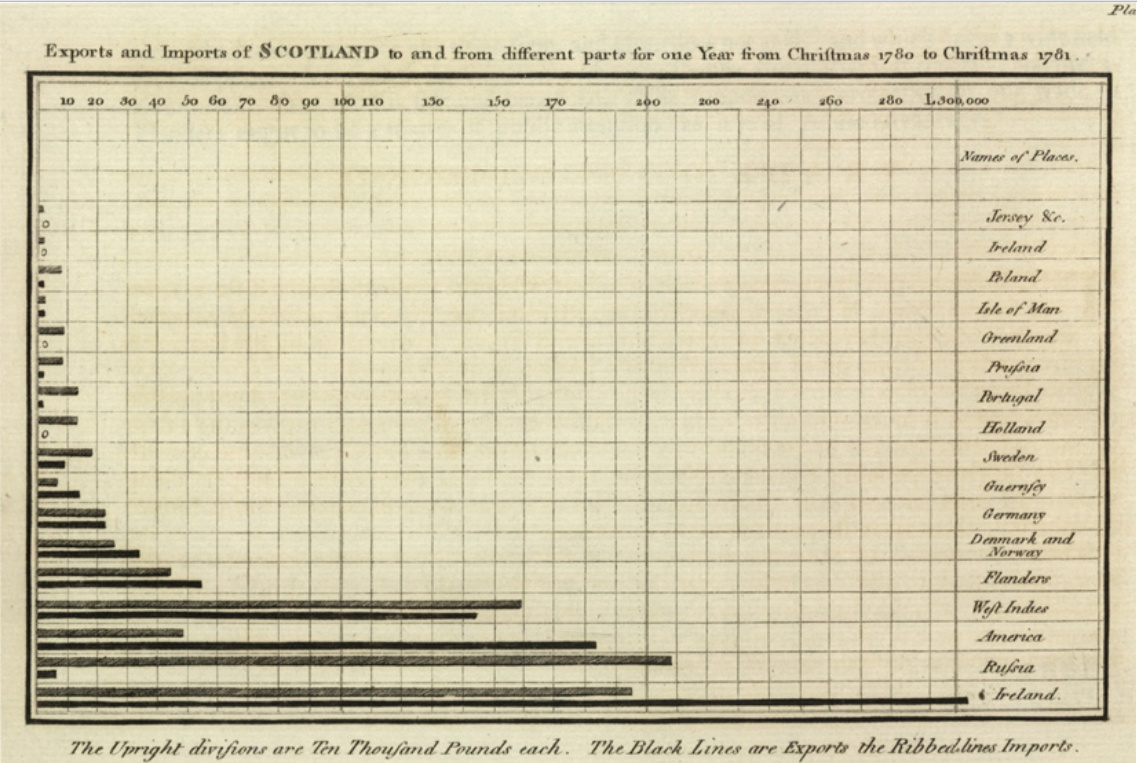
\includegraphics[width=0.75\linewidth]{images/playfair-barchart-1786} 

}

\caption{Commercial and Political Atlas (Atlas Comercial e Político de 1786): cada barra representa as exportações e importações da Escócia para 17 países em 1781}\label{fig:unnamed-chunk-12}
\end{figure}

\begin{figure}

{\centering 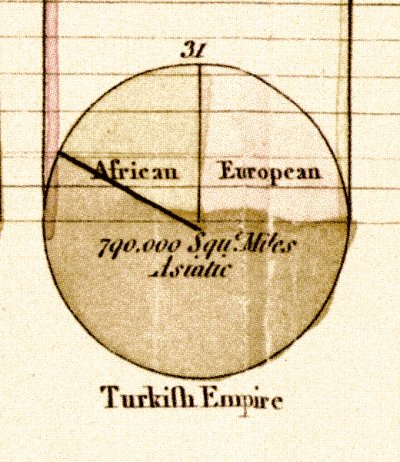
\includegraphics[width=0.75\linewidth]{images/playfair-piechart-1801} 

}

\caption{Statistical Breviary (Breviário Estatístico de 1801): proporção da extensão do Império Turco em diferentes regiões do mundo: Asia, Europa e África, antes de 1789}\label{fig:unnamed-chunk-13}
\end{figure}

1856

A enfermeira inglesa Florence Nightingale (1820-1910) conduziu um trabalho pioneiro ao chegar no hospital militar britânico na Turquia em 1856, estabelecendo uma ordem e um método muito necessários aos registros médicos estatísticos e que indicaram serem as precárias práticas sanitárias o culpado da alta mortalidade \href{https://www.york.ac.uk/depts/maths/histstat/small.htm}{(link)}.

\begin{figure}

{\centering 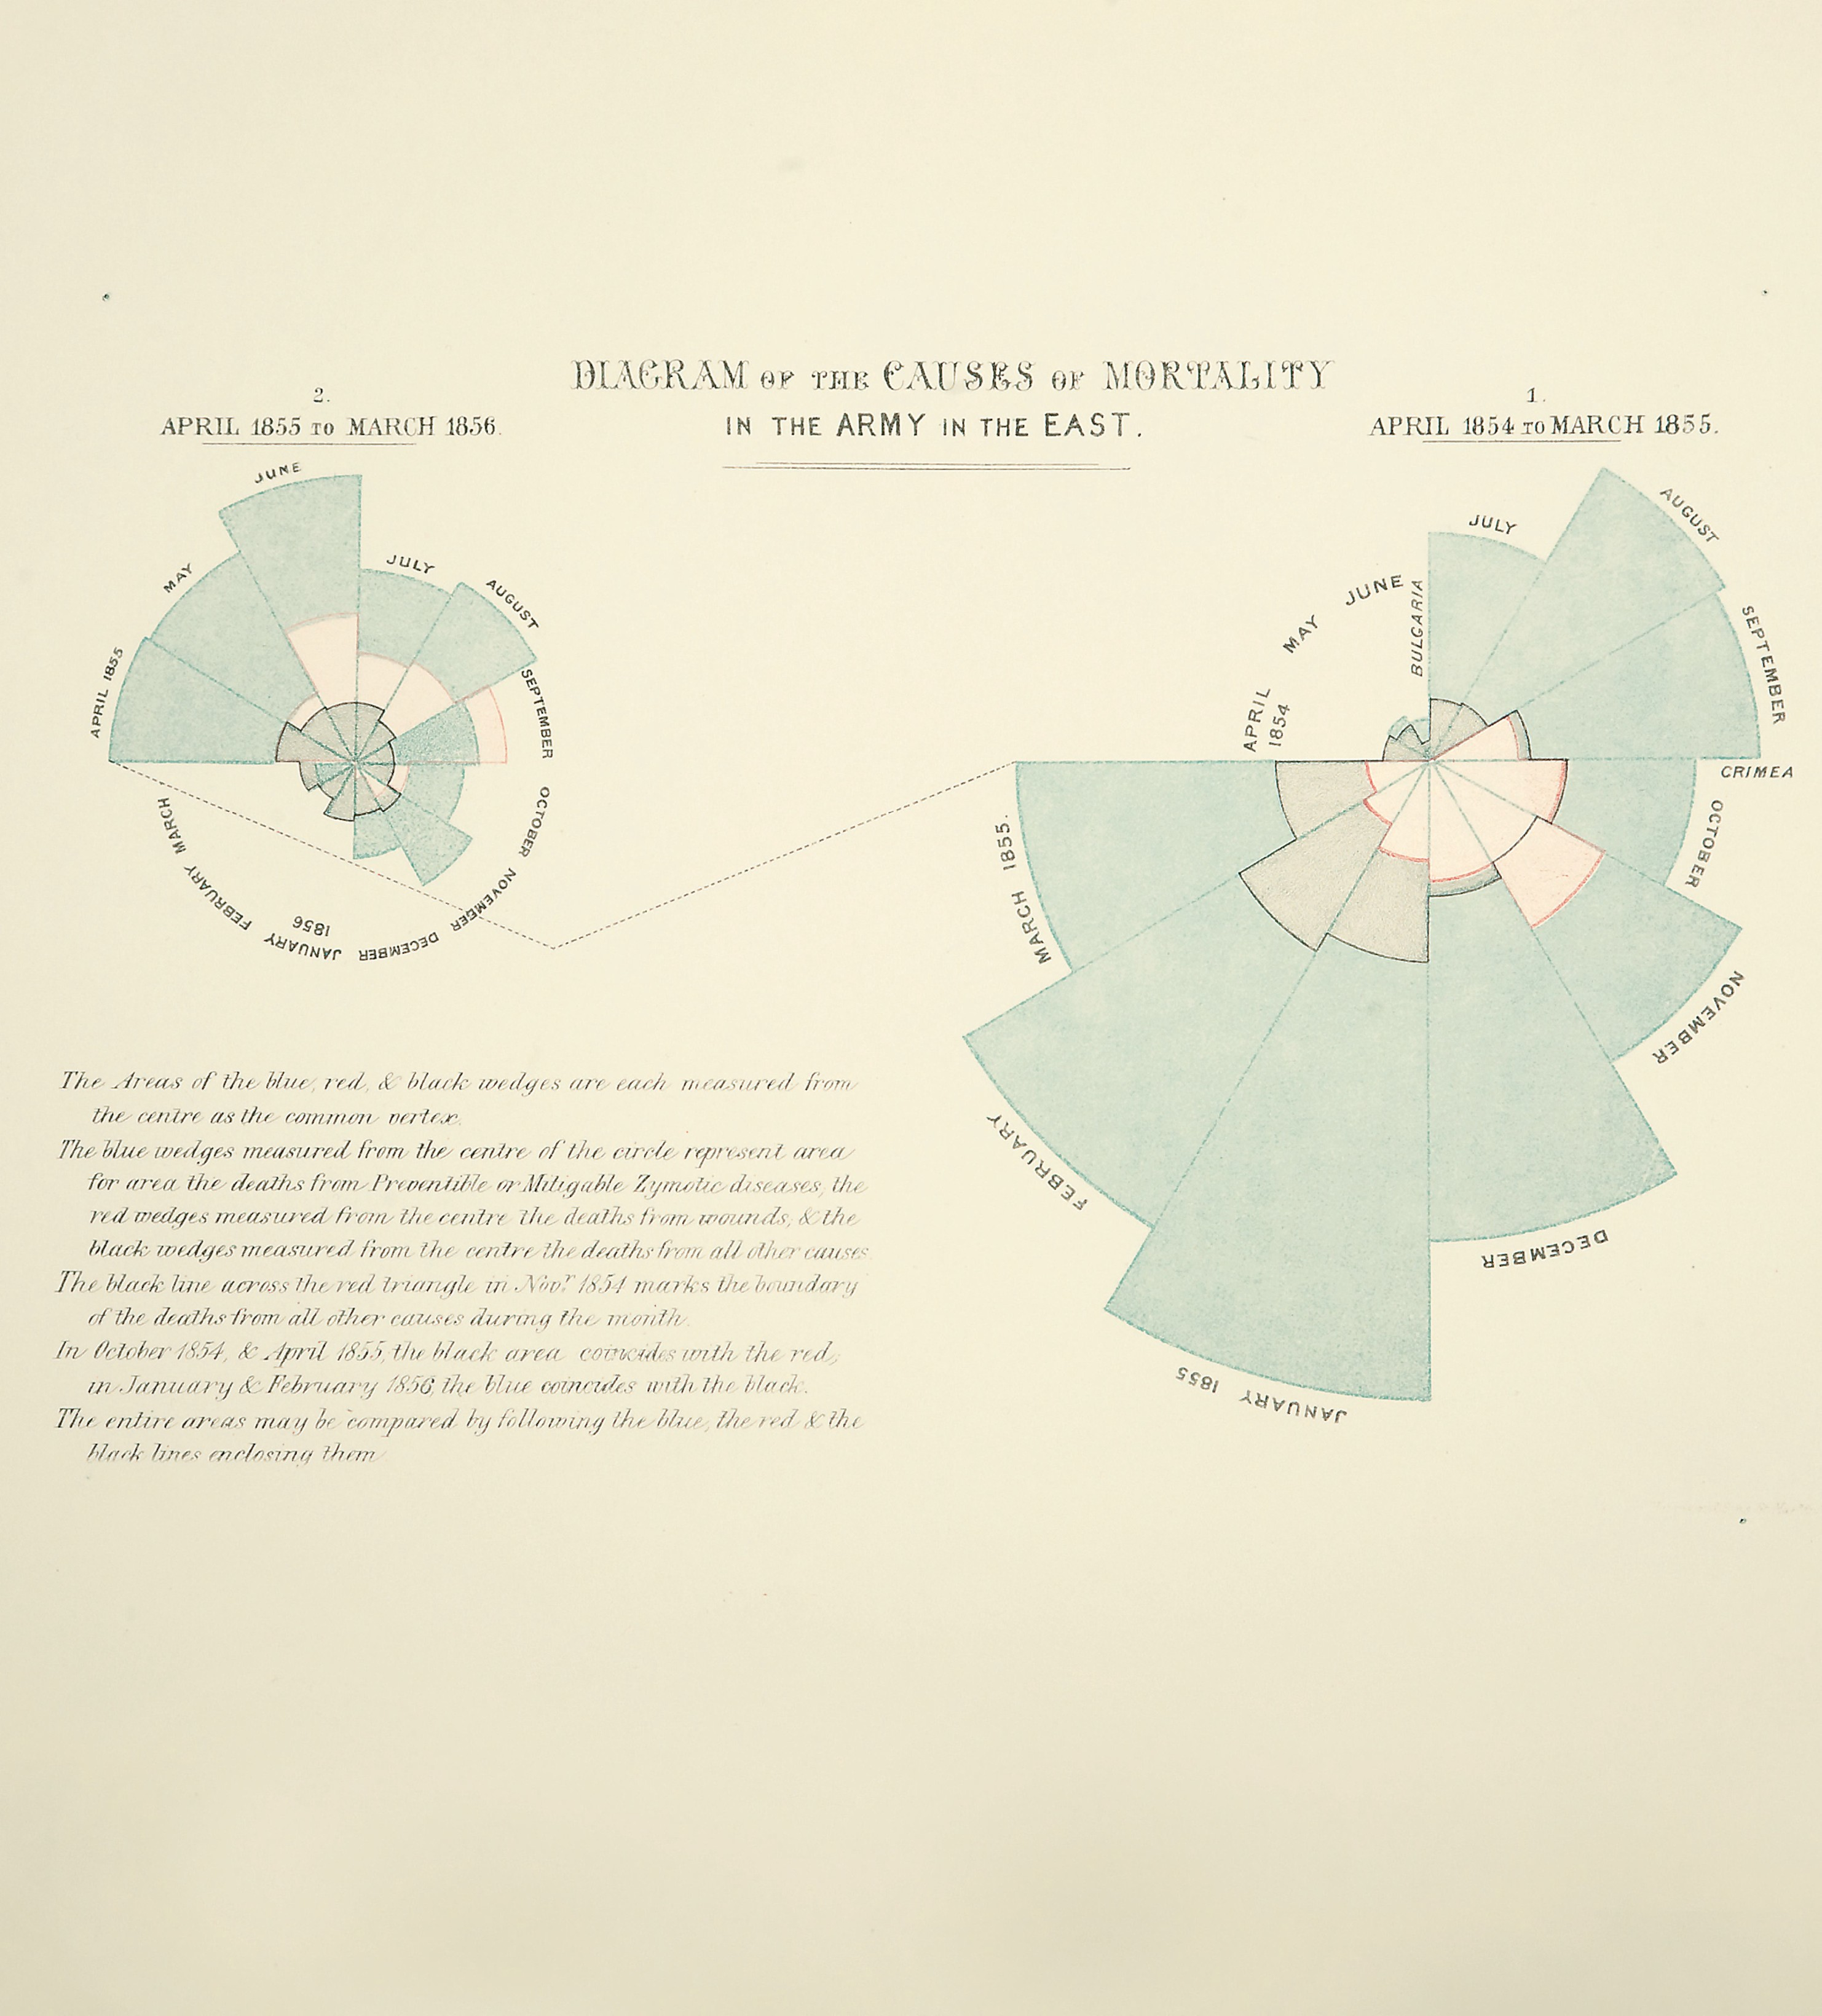
\includegraphics[width=0.75\linewidth]{images/florence-rose-diagram} 

}

\caption{Esse diagrama (coxcomb) feito durante a Guerra da Crimeia foi dividido igualmente em 12 setores, representando os meses do ano, com a área sombreada do setor  de cada mês proporcional à taxa de mortalidade naquele mês. Seu sombreamento com código de cores indicava a causa da morte em cada área do diagrama}\label{fig:unnamed-chunk-14}
\end{figure}

\begin{figure}

{\centering 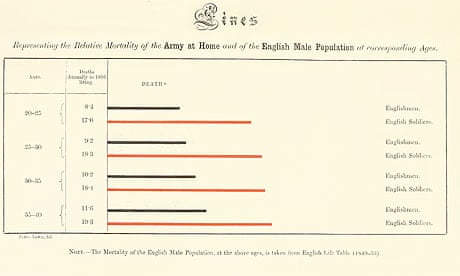
\includegraphics[width=0.75\linewidth]{images/florence-barr} 

}

\caption{Gráfico de barras de Florence Nightingale mostrando as diferenças de mortalidade entre soldados britânicos e a população masculina inglesa geral (civis)}\label{fig:unnamed-chunk-15}
\end{figure}

\hypertarget{nomes-notuxe1veis}{%
\section{Nomes notáveis}\label{nomes-notuxe1veis}}

Karl Pearson (1857-1936) é amplamente considerado o fundador da disciplina moderna de \textbf{estatística}, e também é famoso como um filósofo da ciência, como escritor sobre o darwinismo social e como um dos principais impulsionadores para instalar a eugenia como a ciência social chave. Uma breve biografia de cada um dos pesquisadores a seguir relacionados pode ser obtida em: \href{http://www-history.mcs.st-andrews.ac.uk/BiogIndex.html}{(link)}.

\begin{itemize}
\tightlist
\item
  Niccolò Fontana Tartaglia (Veneza à época, hoje Itália: 1499-1557)
\item
  Girolamo Cardano (Pávia à época, hoje Itália: 1501-1576)
\item
  Galileu Galilei (Florença à época, hoje Itália: 1564-1642)
\item
  Pierre de Fermat (França: 1607-1665)
\item
  Blaise Pascal (França: 1623-1662)
\item
  Jakob Bernoulli (Suíça: 1655-1705)
\item
  Abrahan de Moivre (França: 1667-1754)
\item
  Thomas Bayes (Inglaterra: 1702-1761)
\item
  Pierre-Simon Laplace (França: 1749-1827)
\item
  Johann Carl Friedrich Gauss (Alemanha: 1777-1856)
\item
  Lambert Adolphe Jacques Quételet (França à época, hoje Bélgica: 1796-1874)
\item
  Pafnuti Lvovitch Chebyshev (Rússia: 1821-1894)
\item
  Francis Galton (Inglaterra: 1822-1911)
\item
  Wilhelm Lexis (Alemanha: 1837-1914)
\item
  Thorvald Nicolai Thiele (Dinamarca: 1838-1910)
\item
  Friedrich Robert Helmert (Saxônia: 1843-1917)
\item
  Francis Ysidro Edgeworth (Inglaterra: 1845-1926)
\item
  James Douglas Hamilton Dickson (Escócia: 1849-1931)
\item
  Andrei Andreyevich Markov (Rússia: 1856-1922)
\item
  Aleksandr Mikhailovich Lyapunov (Rússia: 1857-1918)
\item
  Walter Frank Raphael Weldon (Inglaterra: 1860-1906)
\item
  Karl Pearson (Inglaterra: 1857-1936)
\item
  William Seally Gosset (Inglaterra: 1876-1937)
\item
  Ronald Aylmer Fisher (Inglaterra: 1890-1962)
\item
  Andrei Nikolaevich Kolmogorov (Rússia: 1903-1987)
\end{itemize}

\hypertarget{revista-biometrika}{%
\section{Revista Biometrika}\label{revista-biometrika}}

\begin{quote}
``Pretende-se que a \textit{Biometrika} sirva como um meio não apenas de coletar ou publicar, sob um título, dados biológicos de um tipo não coletados sistematicamente ou publicados em outro lugar em qualquer outro periódico, mas também de disseminar um conhecimento de tal teoria estatística para o seu tratamento científico{[}\ldots{]}''
\end{quote}

Em outubro de 1901 foi fundada a \emph{Biometrika, the Journal for the Statistical Study of Biological Problems} (Biometrika, o Jornal para o Estudo Estatístico de Problemas Biológicos) com o propósito de promover a análise estatística de fenômenos biológicos, isto é, a matematização da biologia.

Os fundadores da \emph{Biometrika} foram \emph{Sir} Francis Galton (primo de Charles Darwin), Walter Frank Raphael Weldon e Karl Pearson. A maior parte do trabalho foi feita por Pearson e Weldon, este último focando na edição do conteúdo (ou seja, o aspecto biológico) e o primeiro nos detalhes, incluindo correções de prova. Galton e o eugenista americano Charles Davenport atuaram, respectivamente, como consultor e editor.

Alguns dos tópicos abordados na revista incluem criminologia, botânica, zoologia, epidemiologia e outros aspectos da saúde humana. Na década de 1930, o caráter da \emph{Biometrika} mudou, e ``representou a vanguarda internacional da pesquisa em métodos estatísticos e sua aplicação na ciência e tecnologia'\,', ao invés de focar a hereditariedade.

\emph{Sir} Francis Galton, que serviu como editor da primeira edição (1901), escreveu a Introdução, que incluiu uma declaração de propósito para a revista\\
\href{https://academic.oup.com/biomet/article-abstract/1/1/1/192192?redirectedFrom=fulltext}{(link)}.

\hypertarget{eugenia}{%
\section{Eugenia}\label{eugenia}}

Em 16 de maio de 1883 \emph{Sir} Francis Galton cunhou o termo ``eugenia'', posteriormente descrevendo-o como ``o estudo das agências sob controle social que podem melhorar ou reparar as qualidades raciais das gerações futuras, seja fisicamente ou mentalmente''.

Galton detalha o conceito em seu livro \emph{Inquiries into Human Faculty and its Development}, e recomenda que indivíduos de famílias altamente classificadas em seu sistema de mérito sejam encorajados a se casar cedo e receber incentivos para ter filhos. Ele também condenou os casamentos tardios dentro desse mesmo grupo como ``disgênicos'' ou desvantajosos para a espécie humana.

A palavra ``eugenia'' foi extraída da palavra grega \emph{eu}, que significa bem, e \emph{genos}, que significa prole. Juntos, significa bem-nascido.

Este livro caiu em domínio público e pode ser lido na íntegra online. A caracterização original de eugenia de Galton pode ser encontrada na página 17 desta edição de domínio público (Parte 1 do pdf):

\begin{quote}
``uma breve palavra para expressar a ciência de melhorar o rebanho, que não está de modo algum confinado a questões de acasalamento criterioso, mas que, especialmente no caso do homem, toma conhecimento de todas as influências que tendem, mesmo que em grau remoto, a dar ao raças ou linhagens de sangue mais adequadas uma melhor chance de prevalecer rapidamente sobre os menos adequados do que teriam de outra forma {[}\ldots{]}''(Galton, 1883, p.17)
\end{quote}

Há poucos anos alguns grupos sociais viram no trabalho e opiniões de Fisher endossos ao colonialismo, à supremacia branca e à eugenia.

Outros grupos, todavia, afirmam que Fisher não era racista e eugenista, embora ele achasse que havia diferenças comportamentais e de inteligência entre os grupos humanos.

\begin{figure}

{\centering 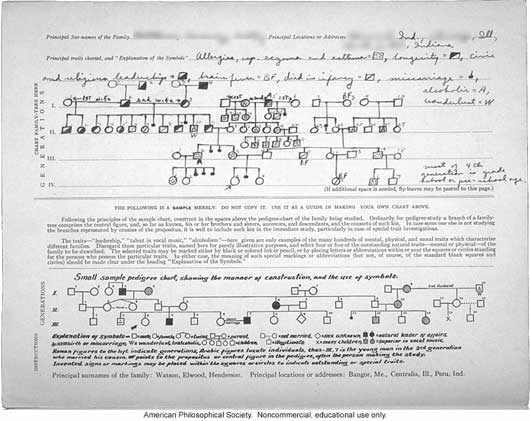
\includegraphics[width=0.75\linewidth]{images/chart_pedigree_allergy2} 

}

\caption{Gráfico de linhagens para alergias}\label{fig:unnamed-chunk-16}
\end{figure}

\begin{figure}

{\centering 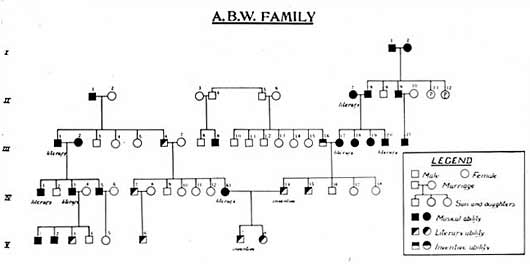
\includegraphics[width=0.75\linewidth]{images/chart_pedigree_music2 (1)} 

}

\caption{Gráfico de linhagens para aptidão musical}\label{fig:unnamed-chunk-17}
\end{figure}

\begin{figure}

{\centering 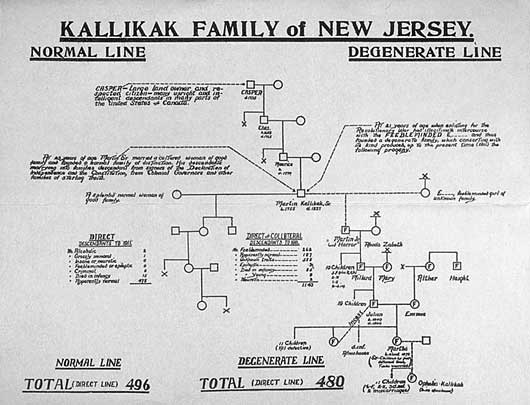
\includegraphics[width=0.75\linewidth]{images/chart_Kallikak_pedigree2} 

}

\caption{Linhas "normais" e "degeneradas" da família Kallikak (New Jersey)}\label{fig:unnamed-chunk-18}
\end{figure}

\begin{figure}

{\centering 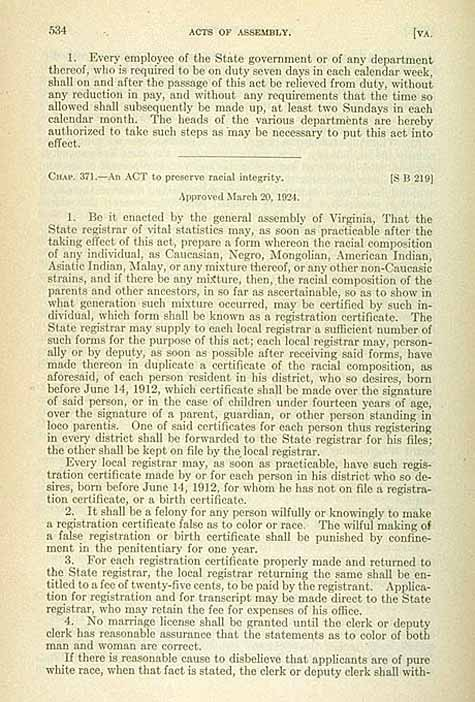
\includegraphics[width=0.75\linewidth]{images/VA_racial_integrity_act2} 

}

\caption{Lei da Inegridade Racia (Virginia, EUA, 1924)}\label{fig:unnamed-chunk-19}
\end{figure}

\begin{figure}

{\centering 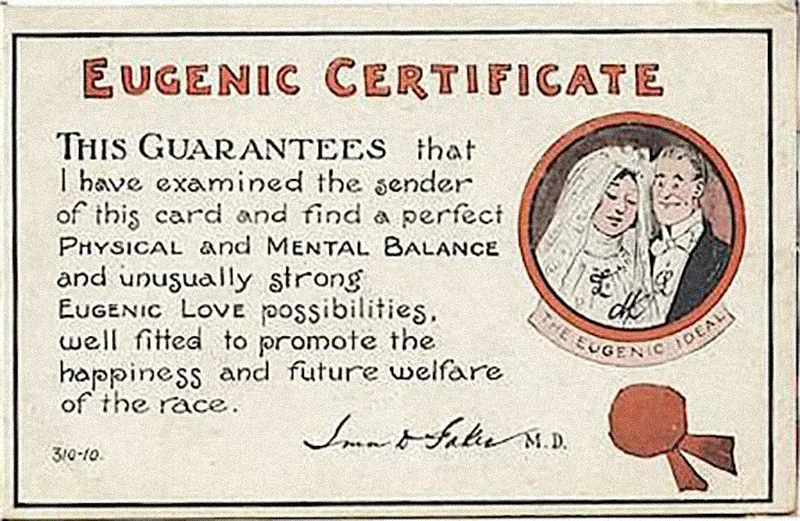
\includegraphics[width=0.75\linewidth]{images/choosing_love_over_eugenics} 

}

\caption{Licença para casamento}\label{fig:unnamed-chunk-20}
\end{figure}

\hypertarget{conceitos_gerais}{%
\chapter{Conceitos gerais}\label{conceitos_gerais}}

\begin{quote}
``Estatística é um conjunto de métodos que se destina a possibilitar a tomada de decisões, face às incertezas{[}\ldots{]}'\,'
\end{quote}

De modo geral, a estatística pode ser dividida em três grandes áreas:

\begin{itemize}
\tightlist
\item
  descritiva;
\item
  probabilidade; e,
\item
  inferencial.
\end{itemize}

\hypertarget{estatuxedstica-descritiva}{%
\section{Estatística descritiva}\label{estatuxedstica-descritiva}}

Nos primeiros trabalhos estatísticos, os dados coletados eram inicialmente apresentados na forma de tabelas e gráficos.

A \textbf{estatística descritiva} se ocupa de tudo o que seja relacionado a dados: coleta, processamento, descrição (seja na forma tabular ou gráfica) e sínteses numéricas (de locação, de dispersão, de repartição) sem inferir coisa alguma além da informação trazida pelos dados. Vem experimentando crescente uso em todas as áreas científicas e desenvolvimento:

\begin{itemize}
\tightlist
\item
  crescente uso de uma abordagem quantitativa em todas as ciências;
\item
  disponibilidade de recursos computacionais;
\item
  quantidade de dados coletados.
\end{itemize}

A palavra \textbf{estatística} pode assumir diferentes significados:

\begin{itemize}
\tightlist
\item
  no singular: \textbf{estatística} \vspace{0.5cm}

  \begin{itemize}
  \tightlist
  \item
    refere-se à ciência que compreende métodos que são usados na coleta, análise, interpretação e apresentação de dados quantitativos ou qualitativos (numéricos ou não); e,
  \item
    denota uma medida ou fórmula específica (tais como uma média, um intervalo de valores, uma taxa de crescimento, um índice).
  \end{itemize}
\item
  no plural: \textbf{estatísticas}

  \begin{itemize}
  \tightlist
  \item
    refere-se a dados coletados de maneira sistemática com um propósito específico definido em qualquer campo de estudo (nesse sentido, as \emph{estatísticas} também podem ser consideradas como agregados de fatos expressos em forma numérica).
  \end{itemize}
\end{itemize}

\hypertarget{estatuxedstica-inferencial}{%
\section{Estatística inferencial}\label{estatuxedstica-inferencial}}

A \textbf{estatística inferencial} tem o objetivo de estabelecer níveis de confiança da tomada de decisão de associar uma estimativa amostral a um parâmetro populacional. Divide-se em estimação e testes de significância.

\begin{quote}
``Dedução e indução são procedimentos racionais que nos levam do já conhecido ao ainda não conhecido; isto é, permitem que adquiramos conhecimentos novos graças a conhecimentos já adquiridos.{[}\ldots{]}''
\end{quote}

Dedução.

Na dedução parte-se de uma verdade já conhecida para demonstrar que ela se aplica a todos os casos particulares iguais. Vai do geral ao particular.

Indução.

Na indução parte-se de alguns casos particulares iguais ou semelhantes para se estipular uma \textbf{lei geral}. Vai do particular ao geral.

Na dedução, dado \textbf{X}, infiro (concluo) \textbf{a}, \textbf{b}, \textbf{c}, \textbf{d}.

Na indução, dados \textbf{a}, \textbf{b}, \textbf{c}, \textbf{d}, infiro (concluo) \textbf{X}.

\begin{quote}
Exemplo: testes de aceleração (0-60 mph) feitos com 6 carros importados em 1999 resultaram nas seguintes medidas: 12,9 s; 16,50 s; 11,30 s; 15,20 s; 18,20 s e 17,70 s. Um estudo descritivo poderia afirmar que:
\end{quote}

\begin{itemize}
\tightlist
\item
  metade dos dados coletados acelera de 0-60 mph em menos de 16,00 s; e
\item
  a aceleração média de 0-60 mph é de 15,30 s.
\end{itemize}

\begin{quote}
Mas, a partir dessa amostra concluir que a aceleração média de \textbf{todos} os carros importados em 1999 seja de 15,30 s; ou, que \textbf{metade} dos carros importados em 1999 acelerem de 0-60 mph em menos de 16,00 s são afirmações que pertencem à \textbf{inferência estatística}.
\end{quote}

\hypertarget{produuxe7uxe3o-de-conhecimento}{%
\section{Produção de conhecimento}\label{produuxe7uxe3o-de-conhecimento}}

\begin{figure}

{\centering \includegraphics[width=1\linewidth]{images/flux-george} 

}

\caption{Fluxograma elementar de um processo de aprendizagem}\label{fig:unnamed-chunk-21}
\end{figure}

Na expansão de qualquer área do conhecimento propomos hipóteses que serão avaliadas mediante a coleta de dados que, depois de analisados, revelarão informações que, eventualmente, nos conduzirão ao afastamento da hipótese original e à proposição de outras, num processo contínuo como, por exemplo:

\begin{enumerate}
\def\labelenumi{(\Alph{enumi})}
\tightlist
\item
\end{enumerate}

\begin{itemize}
\tightlist
\item
  Hipótese (ideia, teoria, conjectura): ``Hoje será um dia como outro qualquer.''
\item
  Dedução: ``Meu carro estará estacionado na garagem, no local de costume.''
\item
  Dados (informação, fatos): ``Meu carro não está lá!''
\item
  Inferência: ``Alguém deve tê-lo levado.''
\end{itemize}

\begin{enumerate}
\def\labelenumi{(\Alph{enumi})}
\setcounter{enumi}{1}
\tightlist
\item
\end{enumerate}

\begin{itemize}
\tightlist
\item
  Hipótese (ideia, teoria, conjectura): ``Meu carro foi roubado!''
\item
  Dedução: ``Meu carro não estará no local de costume.''
\item
  Dados (informação, fatos): ``Meu carro está lá!''
\item
  Inferência: ``Alguém deve tê-lo levado e devolvido.''
\end{itemize}

\begin{enumerate}
\def\labelenumi{(\Alph{enumi})}
\setcounter{enumi}{2}
\tightlist
\item
\end{enumerate}

\begin{itemize}
\tightlist
\item
  Hipótese (ideia, teoria, conjectura): ``Um ladrão pegou e trouxe de volta.''
\item
  Dedução: ``Meu carro foi arrombado.''
\item
  Dados (informação, fatos): ``Meu carro está intacto e o alarme está desligado.''
\item
  Inferência: ``Alguém que tenha as chaves deve tê-lo levado.''
\end{itemize}

\begin{enumerate}
\def\labelenumi{(\Alph{enumi})}
\setcounter{enumi}{3}
\tightlist
\item
\end{enumerate}

\begin{itemize}
\tightlist
\item
  Hipótese (ideia, teoria, conjectura): ``Minha esposa usou meu carro.''
\item
  Dedução: ``Ela provavelmente deixou um bilhete.''
\item
  Dados (informação, fatos): ``Sim, aqui está o bilhete.''
\item
  Inferência: ``Minha hipótese estava correta.''
\end{itemize}

Uma investigação científica deve envolver, em linhas gerais:

\begin{itemize}
\tightlist
\item
  observação dos fatos;
\item
  descrição das características essenciais, segundo o que se obteve através da observação;
\item
  explicação dessas características descritivas;
\item
  previsão; e,
\item
  decisão pertinente à investigação.
\end{itemize}

O planejamento de uma pesquisa deve envolver, em linhas gerais:

\begin{itemize}
\tightlist
\item
  definição do \textit{universo}: é necessário delimitar claramente, no tempo e espaço, o âmbito do inquérito, definindo, em termos precisos, o \textit{universo} a ser trabalhado;
\item
  exame das informações disponíveis: deve-se reunir todo o material existente: mapas, artigos, livros, relatórios relativos a levantamentos semelhantes;
\item
  tipos de levantamentos: completo ou amostral;
\item
  prazo;
\item
  custo;
\item
  precisão.
\end{itemize}

\hypertarget{populauxe7uxe3o-universo-amostra}{%
\section{População (universo) \& amostra}\label{populauxe7uxe3o-universo-amostra}}

\begin{figure}

{\centering 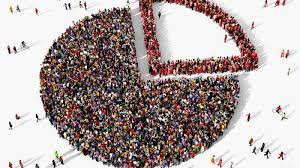
\includegraphics[width=1\linewidth]{images/amostragem} 

}

\caption{Universo e amostra}\label{fig:unnamed-chunk-22}
\end{figure}

Quase que, invariavelmente, em todo ramo de conhecimento, o pesquisador esbarra em uma séria de limitações das mais variadas ordens (econômica, técnica, ética, geográfica, temporal,\ldots) que impossibilitam o estudo dos dados e informações associados a todos os casos existentes (\textbf{população ou universo}).

Por essa razão, através de um procedimento estatístico denominado de amostragem, estuda-se uma população (universo) a partir de uma amostra. Amostra é, portanto, um subconjunto finito e representativo da população (universo), extraído de modo sistemático (planejado).

\hypertarget{paruxe2metros-e-estatuxedsticas}{%
\section{Parâmetros e estatísticas}\label{paruxe2metros-e-estatuxedsticas}}

É comum a adoção de letras gregas para as características descritivas que se referirem à poúlação (universo) e letras do alfabeto latino para aquelas relativas à amostra extraída:

\begin{longtable}[]{@{}lll@{}}
\toprule
Característica estudada & Notação populacional & Notação amostral \\
\midrule
\endhead
Número de elementos & N & n \\
Média & \(\mu\) & \(\stackrel{-}{x}\) \\
Variância & \(\sigma^{2}\) & \({s}^{2}\) \\
Desvio padrão & \(\sigma\) & s \\
Proporção & \(\Pi\) & p \\
\bottomrule
\end{longtable}

\begin{figure}

{\centering 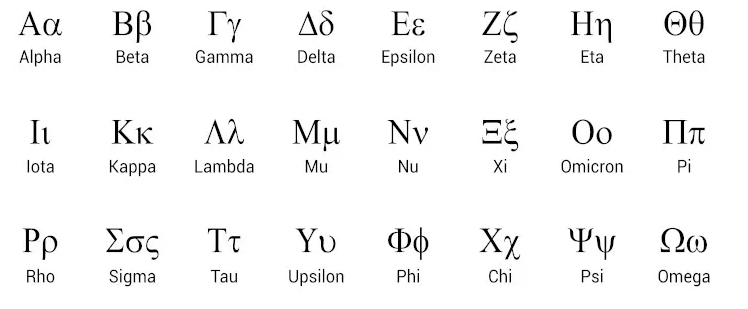
\includegraphics[width=1\linewidth]{images/alf_grego} 

}

\caption{Alfabeto grego}\label{fig:unnamed-chunk-23}
\end{figure}

\hypertarget{tipos-de-variuxe1veis}{%
\section{Tipos de variáveis}\label{tipos-de-variuxe1veis}}

Variáveis quantitativas

\begin{itemize}
\tightlist
\item
  contínuas: são os dados com maior potencial de produzir informação significativa dentre todos: comprimentos, áreas, pesos, densidades; e,
\item
  discretas: são dados com um pouco menos de informação que os de natureza contínua mas possuem mais informação que dados qualitativos: número de andares de um prédio, de degraus de uma escada, número de filhos de um casal.
\end{itemize}

Variáveis qualitativas

\begin{itemize}
\tightlist
\item
  ordinais: apresentam um pouco mais de informação que os dados qualitativos puramente nominais na medida que suas classes podem ser interpretadas como possuindo um ordenamento inerente: padrão construtivo (baixo, médio, alto), classe econômica de rendimento (baixa, média, alta), nível de escolaridade (fundamental, médio e superior); e,
\item
  nominais: são dados a menor quantidade de informação: sexo, cor, códigos postais de cidades;
\end{itemize}

Codificação de variáveis qualitativas

\begin{itemize}
\tightlist
\item
  binárias: pela associação de valores numéricos: 0 ou 1 a uma variável qualitativa nominal que se apresente com apenas dois aspectos: sim ou não, ausência ou presença. Pela composição de mais variáveis binárias pode-se codificar variáveis que possuam um número maior de classes; e,
\item
  \emph{proxy}: pela associação de valores numéricos contínuos que guardam ``correlação'\,' com as classes da variável qualitativa nominal.
\end{itemize}

\begin{figure}

{\centering 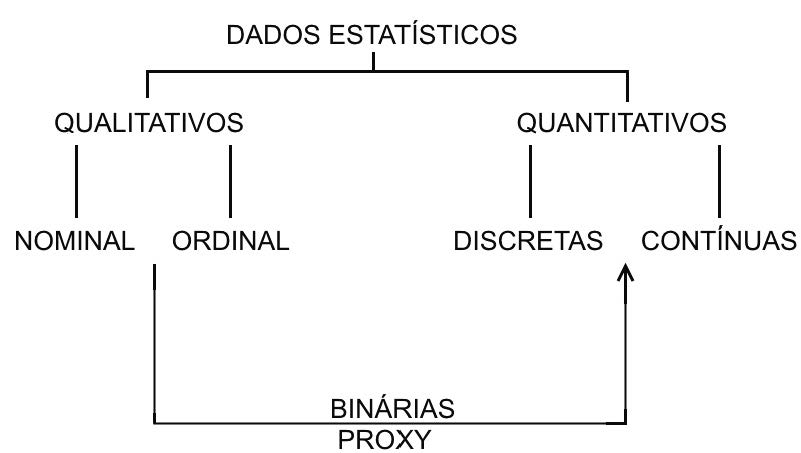
\includegraphics[width=0.75\linewidth]{images/tipos_variaveis} 

}

\caption{Tipos e codificações de variáveis }\label{fig:unnamed-chunk-24}
\end{figure}

  \bibliography{book.bib,packages.bib}

\end{document}
